\section{Exploration}
\label{sec:exploration}

While collecting these data, it was helpful to explore them, in order to
discover features that could characterize places and help cluster them into
similar groups.

\subsection{Time}

The time at which check-ins occur is undoubtedly a important variable. For
instance, \textcite{UrbanStory12} perform topic modelling from the text of
check-in tweets and show that various topics exhibit daily or weekly
patterns. Likewise, \textcite{TimeCluster13} cluster cells of a rectangular
grid according to their repartition of check-ins over categories and time of
day.

Thus we first look at when check-ins are performed through the day
\autoref{fig:daily_checkin} or the week \autoref{fig:weekly_checkin}, and how it
differ whether we consider New York, the city that never sleeps, or Helsinki.

But these patterns do not affect all venues uniformly. Taking Paris as an
example, we can summarize each venue's activity by an histogram with 3 or 4
four hours bins. Then, running $k$-means algorithm with $k=5$, we obtained the
clusters depicted in \autoref{fig:day_cluster}. We observe that they have
the same characteristic shape with one peak during the day and relatively low
activity the rest of the time. We repeat these in all the cities to determine
if these clusters are universal. As showed in \autoref{fig:time_cluster_size},
it is the case with 4-hours bins, but 3-hours clusters exhibit slight
variations across cities of our dataset.

\begin{figure}[hbt]
    \begin{subfigure}[b]{\textwidth}
    \centering
    \iftoggle{EXTERNALPGF}{%
        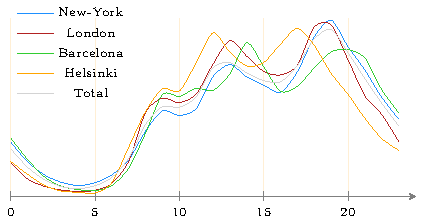
\includegraphics[width=\textwidth]{daily_checkin}
    }{%
        \begin{tikzpicture}
	\begin{axis}[xmin=0, xmax=24,
            unit vector ratio*=1 1.2,
	    axis y line=none,
            ymin=0, ymax=8.8,
            % title={Hourly check-ins frequency through the day},
            % xlabel={hour},
            % ylabel={percentage},
            legend style={at={(0.0,0.8)},anchor=west,draw=none,fill=none},
            grid=major
		]
\addplot[DodgerBlue,thin, smooth]table [x={time}, y={freq}] {newyork_day.dat};
\addlegendentry{New-York}
\addplot[FireBrick,thin, smooth]table [x={time}, y={freq}] {london_day.dat};
\addlegendentry{London}
\addplot[LimeGreen,thin, smooth]table [x={time}, y={freq}] {barcelona_day.dat};
\addlegendentry{Barcelona}
\addplot[Orange,thin, smooth]table [x={time}, y={freq}] {helsinki_day.dat};
\addlegendentry{Helsinki}
\addplot[LightGray,thin, smooth]table [x={time}, y={freq}] {global_day.dat};
\addlegendentry{Total}
\end{axis}
\end{tikzpicture}

    }
	\caption[Pattern of check-in during the day]{Hourly check-ins frequency
		during the day. The activity is at its lowest around 5 \am\ and after
		that, there are three peaks: one when people go to work in the morning,
		one in the middle of the day and the last one at the end of the
		evening. Yet, depending of the city, these peaks do not happen at the
		same time, nor with the same intensity. Therefore, instead of working
		directly the raw values of features, we use the number of standard
		deviation or \emph{z-score}.\label{fig:daily_checkin}}
    \end{subfigure}

    \begin{subfigure}[b]{\textwidth}
    \centering
    \iftoggle{EXTERNALPGF}{%
        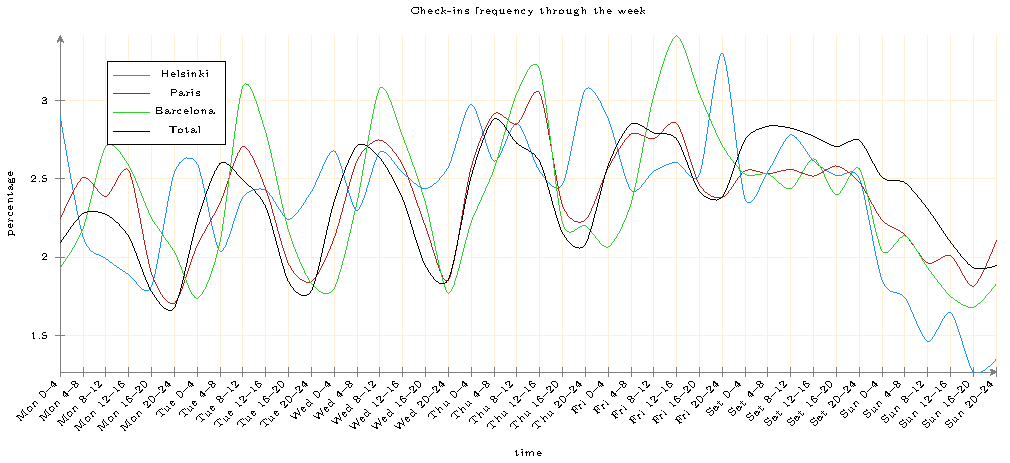
\includegraphics[width=\textwidth]{weekly_checkin}
    }{%
        %Mon 0--4, % Mon 4--8, Mon 8--12, % Mon 12--16, Mon 16--20, % Mon 20--24, Tue 0--4, % Tue 4--8, Tue 8--12, % Tue 12--16, Tue 16--20, % Tue 20--24, Wed 0--4, % Wed 4--8, Wed 8--12, % Wed 12--16, Wed 16--20, % Wed 20--24, Thu 0--4, % Thu 4--8, Thu 8--12, % Thu 12--16, Thu 16--20, % Thu 20--24, Fri 0--4, % Fri 4--8, Fri 8--12, % Fri 12--16, Fri 16--20, % Fri 20--24, Sat 0--4, % Sat 4--8, Sat 8--12, % Sat 12--16, Sat 16--20, % Sat 20--24, Sun 0--4, % Sun 4--8, Sun 8--12, % Sun 12--16, Sun 16--20, % Sun 20--24
\begin{tikzpicture}
    \begin{axis}[x={11},
            % title={Check-ins frequency through the week},
            % xlabel={time},
            % ylabel={percentage},
		    ymax=3.4,axis y line=none,
            legend
	    style={at={(0.76,0.00)},anchor=south,draw=none,fill=none,font=\Large,cells={line width=2pt}},
            x tick label style={rotate=45,anchor=east,font=\large},
            grid=major,
	    major grid style={line width=0.03pt, PapayaWhip},
	    xticklabels={%
		    Mon 0--4,,
		    % Mon 4--8,
		    Mon 8--12,,
		    % Mon 12--16,
		    Mon 16--20,,
		    % Mon 20--24,
		    Tue 0--4,,
		    % Tue 4--8,
		    Tue 8--12,,
		    % Tue 12--16,
		    Tue 16--20,,
		    % Tue 20--24,
		    Wed 0--4,,
		    % Wed 4--8,
		    Wed 8--12,,
		    % Wed 12--16,
		    Wed 16--20,,
		    % Wed 20--24,
		    Thu 0--4,,
		    % Thu 4--8,
		    Thu 8--12,,
		    % Thu 12--16,
		    Thu 16--20,,
		    % Thu 20--24,
		    Fri 0--4,,
		    % Fri 4--8,
		    Fri 8--12,,
		    % Fri 12--16,
		    Fri 16--20,,
		    % Fri 20--24,
		    Sat 0--4,,
		    % Sat 4--8,
		    Sat 8--12,,
		    % Sat 12--16,
		    Sat 16--20,,
		    % Sat 20--24,
		    Sun 0--4,,
		    % Sun 4--8,
		    Sun 8--12,,
		    % Sun 12--16,
		    Sun 16--20,,
		    % Sun 20--24
	    },
            xtick={0,...,41},
        ]
\addplot[DodgerBlue, smooth]table [x={time}, y={freq}] {newyork_week.dat};
\addlegendentry{New-York}
\addplot[FireBrick, smooth]table [x={time}, y={freq}] {london_week.dat};
\addlegendentry{London}
\addplot[LimeGreen, smooth]table [x={time}, y={freq}] {barcelona_week.dat};
\addlegendentry{Barcelona}
\addplot[Orange, smooth]table [x={time}, y={freq}] {helsinki_week.dat};
\addlegendentry{Helsinki}
\addplot[LightGray, smooth]table [x={time}, y={freq}] {global_week.dat};
\addlegendentry{Total}
% \addplot[DodgerBlue, smooth]table [x={time}, y={freq}] {helsinki_week.dat};
% \addlegendentry{Helsinki}
% \addplot[FireBrick, smooth]table [x={time}, y={freq}] {paris_week.dat};
% \addlegendentry{Paris}
% \addplot[LimeGreen, smooth]table [x={time}, y={freq}] {barcelona_week.dat};
% \addlegendentry{Barcelona}
% \addplot[Black, smooth]table [x={time}, y={freq}] {global_week.dat};
% \addlegendentry{Total}
\end{axis}
\end{tikzpicture}

    }
	\caption[Pattern of check-in during the week]{Four-hour check-in frequency
	during the week. We observe a day/night cycle, which becomes less
	distinctive as the weekend is approaching and disappears on
	Saturday.\label{fig:weekly_checkin}}
    \end{subfigure}
    \caption{Check-ins temporal pattern.\label{fig:time_checkin}}
\end{figure}

\begin{figure}[hbt]
    \begin{subfigure}[b]{\textwidth}
    \centering
    \iftoggle{EXTERNALPGF}{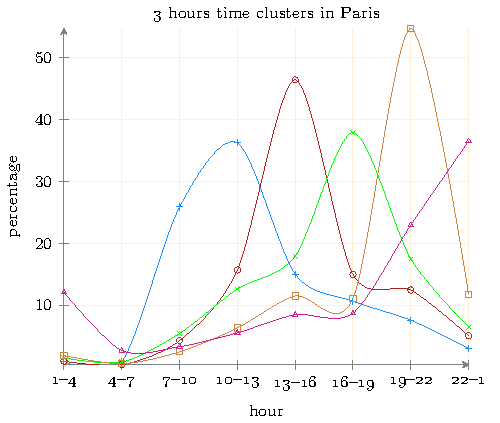
\includegraphics[width=\textwidth]{day_cluster_3h}}{\begin{tikzpicture}
	\begin{axis}[%
            title={3 hours time clusters in Paris},
            xlabel={hour},
            ylabel={percentage},
            % legend style={at={(0.05,0.8)},anchor=west},
            grid=major,
            xticklabels={,1--4, 4--7, 7--10, 10--13, 13--16, 16--19, 19--22, 22--1},
		]
\addplot[DodgerBlue , thin, smooth, mark size={1.5pt}, mark=+ ]table [x index=0, y index=1] {paris_cluster_day_3h.dat};
\addplot[FireBrick  , thin, smooth, mark size={1.5pt}, mark=o ]table      [x index=0, y index=2] {paris_cluster_day_3h.dat};
\addplot[Lime       , thin, smooth, mark size={1.5pt}, mark=x ]table [x index=0, y index=3] {paris_cluster_day_3h.dat};
\addplot[Peru       , thin, smooth, mark size={1.5pt}, mark=square ]table [x index=0, y index=4] {paris_cluster_day_3h.dat};
\addplot[VioletRed  , thin, smooth, mark size={1.5pt}, mark=triangle      ]table [x index=0, y index=5] {paris_cluster_day_3h.dat};
\end{axis}
\end{tikzpicture}


}
    \end{subfigure}

    \begin{subfigure}[b]{\textwidth}
    \centering
    \iftoggle{EXTERNALPGF}{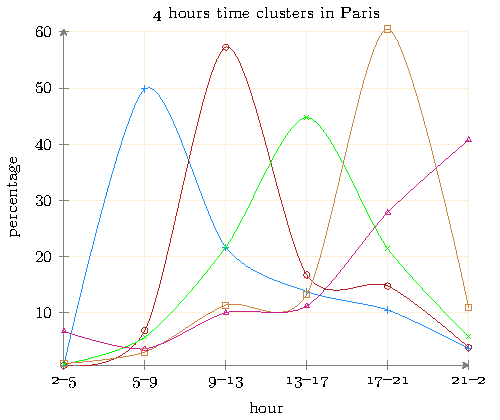
\includegraphics[width=\textwidth]{day_cluster_4h}}{\begin{tikzpicture}
	\begin{axis}[%
            title={4 hours time clusters in Paris},
            xlabel={hour},
            ylabel={percentage},
            % legend style={at={(0.05,0.8)},anchor=west},
            grid=major,
            xticklabels={,2--5,5--9,9--13,13--17,17--21,21--2}
		]
\addplot[DodgerBlue , thin, smooth, mark size={1.5pt}, mark=+ ]table [x index=0, y index=1] {paris_cluster_day_4h.dat};
\addplot[FireBrick  , thin, smooth, mark size={1.5pt}, mark=o ]table      [x index=0, y index=2] {paris_cluster_day_4h.dat};
\addplot[Lime       , thin, smooth, mark size={1.5pt}, mark=x ]table [x index=0, y index=3] {paris_cluster_day_4h.dat};
\addplot[Peru       , thin, smooth, mark size={1.5pt}, mark=square ]table [x index=0, y index=4] {paris_cluster_day_4h.dat};
\addplot[VioletRed  , thin, smooth, mark size={1.5pt}, mark=triangle      ]table [x index=0, y index=5] {paris_cluster_day_4h.dat};
\end{axis}
\end{tikzpicture}

}
    \end{subfigure}
    \caption[Venues clustered by time of check-ins]{Venues clustered by time
    of check-ins. \label{fig:day_cluster}}
\end{figure}

\newgeometry{vmargin=0.65cm,hmargin=1.4cm}
\begin{figure}[p]
	\centering
    \begin{subfigure}[b]{0.35\textwidth}
    \centering
    \iftoggle{EXTERNALPGF}{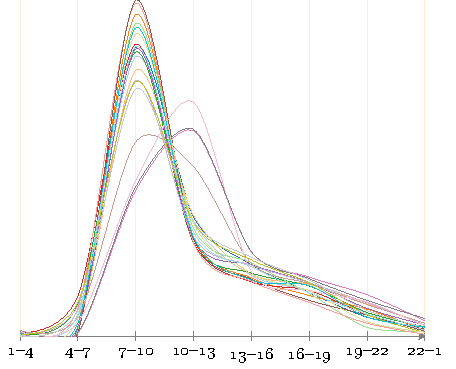
\includegraphics[height=0.18\textheight]{cluster_day_3h_cl1}}{\begin{tikzpicture}
	\begin{axis}[%
			axis y line=none,
            % title={3 hours Cluster 1 in all cities},
            % xlabel={hour},
            % ylabel={percentage},
            grid=major,
            xticklabels={,1--4, 4--7, 7--10, 10--13, 13--16, 16--19, 19--22, 22--1},
		]
\addplot[ck1, thin, smooth] table[x index=0, y index=1] {amsterdam_cluster_day_3h.dat};
\addplot[ck2, thin, smooth,] table[x index=0, y index=1]{atlanta_cluster_day_3h.dat};
\addplot[ck3, thin, smooth,] table[x index=0, y index=1]{barcelona_cluster_day_3h.dat};
\addplot[ck4, thin, smooth,] table[x index=0, y index=1]{berlin_cluster_day_3h.dat};
\addplot[ck5, thin, smooth,] table[x index=0, y index=1]{chicago_cluster_day_3h.dat};
\addplot[ck6, thin, smooth,] table[x index=0, y index=1]{helsinki_cluster_day_3h.dat};
\addplot[ck7, thin, smooth,] table[x index=0, y index=1]{houston_cluster_day_3h.dat};
\addplot[ck8, thin, smooth,] table[x index=0, y index=1]{indianapolis_cluster_day_3h.dat};
\addplot[ck9, thin, smooth,] table[x index=0, y index=1]{london_cluster_day_3h.dat};
\addplot[ck10, thin, smooth,] table[x index=0, y index=1]{losangeles_cluster_day_3h.dat};
\addplot[ck11, thin, smooth,] table[x index=0, y index=1]{moscow_cluster_day_3h.dat};
\addplot[ck12, thin, smooth,] table[x index=0, y index=1]{newyork_cluster_day_3h.dat};
\addplot[ck13, thin, smooth,] table[x index=0, y index=1]{paris_cluster_day_3h.dat};
\addplot[ck14, thin, smooth,] table[x index=0, y index=1]{prague_cluster_day_3h.dat};
\addplot[ck15, thin, smooth,] table[x index=0, y index=1]{rome_cluster_day_3h.dat};
\addplot[ck16, thin, smooth,] table[x index=0, y index=1]{sanfrancisco_cluster_day_3h.dat};
\addplot[ck17, thin, smooth,] table[x index=0, y index=1]{seattle_cluster_day_3h.dat};
\addplot[ck18, thin, smooth,] table[x index=0, y index=1]{stlouis_cluster_day_3h.dat};
\addplot[ck19, thin, smooth,] table[x index=0, y index=1]{stockholm_cluster_day_3h.dat};
\addplot[ck20, thin, smooth,] table[x index=0, y index=1]{washington_cluster_day_3h.dat};
\end{axis}
\end{tikzpicture}
}
    \end{subfigure}~
    \begin{subfigure}[b]{0.35\textwidth}
    \centering
    \iftoggle{EXTERNALPGF}{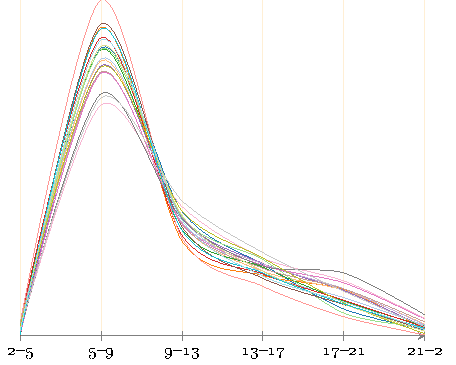
\includegraphics[height=0.18\textheight]{cluster_day_4h_cl1}}{\begin{tikzpicture}
	\begin{axis}[%
            title={ 4 hours Cluster 1 in all cities},
            xlabel={hour},
            ylabel={percentage},
            grid=major,
            xticklabels={,2--5,5--9,9--13,13--17,17--21,21--2}
		]
\addplot[ck1, thin, smooth] table[x index=0, y index=1] {amsterdam_cluster_day_4h.dat};
\addplot[ck2, thin, smooth,] table[x index=0, y index=1]{atlanta_cluster_day_4h.dat};
\addplot[ck3, thin, smooth,] table[x index=0, y index=1]{barcelona_cluster_day_4h.dat};
\addplot[ck4, thin, smooth,] table[x index=0, y index=1]{berlin_cluster_day_4h.dat};
\addplot[ck5, thin, smooth,] table[x index=0, y index=1]{chicago_cluster_day_4h.dat};
\addplot[ck6, thin, smooth,] table[x index=0, y index=1]{helsinki_cluster_day_4h.dat};
\addplot[ck7, thin, smooth,] table[x index=0, y index=1]{houston_cluster_day_4h.dat};
\addplot[ck8, thin, smooth,] table[x index=0, y index=1]{indianapolis_cluster_day_4h.dat};
\addplot[ck9, thin, smooth,] table[x index=0, y index=1]{london_cluster_day_4h.dat};
\addplot[ck10, thin, smooth,] table[x index=0, y index=1]{losangeles_cluster_day_4h.dat};
\addplot[ck11, thin, smooth,] table[x index=0, y index=1]{moscow_cluster_day_4h.dat};
\addplot[ck12, thin, smooth,] table[x index=0, y index=1]{newyork_cluster_day_4h.dat};
\addplot[ck13, thin, smooth,] table[x index=0, y index=1]{paris_cluster_day_4h.dat};
\addplot[ck14, thin, smooth,] table[x index=0, y index=1]{prague_cluster_day_4h.dat};
\addplot[ck15, thin, smooth,] table[x index=0, y index=1]{rome_cluster_day_4h.dat};
\addplot[ck16, thin, smooth,] table[x index=0, y index=1]{sanfrancisco_cluster_day_4h.dat};
\addplot[ck17, thin, smooth,] table[x index=0, y index=1]{seattle_cluster_day_4h.dat};
\addplot[ck18, thin, smooth,] table[x index=0, y index=1]{stlouis_cluster_day_4h.dat};
\addplot[ck19, thin, smooth,] table[x index=0, y index=1]{stockholm_cluster_day_4h.dat};
\addplot[ck20, thin, smooth,] table[x index=0, y index=1]{washington_cluster_day_4h.dat};
\end{axis}
\end{tikzpicture}
}
    \end{subfigure}

    \begin{subfigure}[b]{0.35\textwidth}
    \centering
    \iftoggle{EXTERNALPGF}{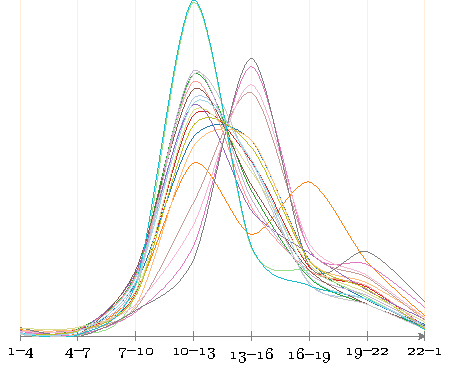
\includegraphics[height=0.18\textheight]{cluster_day_3h_cl2}}{\begin{tikzpicture}
	\begin{axis}[%
			axis y line=none,
            % title={3 hours Cluster 2 in all cities},
            % xlabel={hour},
            % ylabel={percentage},
            grid=major,
            xticklabels={,1--4, 4--7, 7--10, 10--13, 13--16, 16--19, 19--22, 22--1},
		]
\addplot[ck1, thin, smooth] table[x index=0, y index=2] {amsterdam_cluster_day_3h.dat};
\addplot[ck2, thin, smooth,] table[x index=0, y index=2]{atlanta_cluster_day_3h.dat};
\addplot[ck3, thin, smooth,] table[x index=0, y index=2]{barcelona_cluster_day_3h.dat};
\addplot[ck4, thin, smooth,] table[x index=0, y index=2]{berlin_cluster_day_3h.dat};
\addplot[ck5, thin, smooth,] table[x index=0, y index=2]{chicago_cluster_day_3h.dat};
\addplot[ck6, thin, smooth,] table[x index=0, y index=2]{helsinki_cluster_day_3h.dat};
\addplot[ck7, thin, smooth,] table[x index=0, y index=2]{houston_cluster_day_3h.dat};
\addplot[ck8, thin, smooth,] table[x index=0, y index=2]{indianapolis_cluster_day_3h.dat};
\addplot[ck9, thin, smooth,] table[x index=0, y index=2]{london_cluster_day_3h.dat};
\addplot[ck10, thin, smooth,] table[x index=0, y index=2]{losangeles_cluster_day_3h.dat};
\addplot[ck11, thin, smooth,] table[x index=0, y index=2]{moscow_cluster_day_3h.dat};
\addplot[ck12, thin, smooth,] table[x index=0, y index=2]{newyork_cluster_day_3h.dat};
\addplot[ck13, thin, smooth,] table[x index=0, y index=2]{paris_cluster_day_3h.dat};
\addplot[ck14, thin, smooth,] table[x index=0, y index=2]{prague_cluster_day_3h.dat};
\addplot[ck15, thin, smooth,] table[x index=0, y index=2]{rome_cluster_day_3h.dat};
\addplot[ck16, thin, smooth,] table[x index=0, y index=2]{sanfrancisco_cluster_day_3h.dat};
\addplot[ck17, thin, smooth,] table[x index=0, y index=2]{seattle_cluster_day_3h.dat};
\addplot[ck18, thin, smooth,] table[x index=0, y index=2]{stlouis_cluster_day_3h.dat};
\addplot[ck19, thin, smooth,] table[x index=0, y index=2]{stockholm_cluster_day_3h.dat};
\addplot[ck20, thin, smooth,] table[x index=0, y index=2]{washington_cluster_day_3h.dat};
\end{axis}
\end{tikzpicture}
}
    \end{subfigure}~
    \begin{subfigure}[b]{0.35\textwidth}
    \centering
    \iftoggle{EXTERNALPGF}{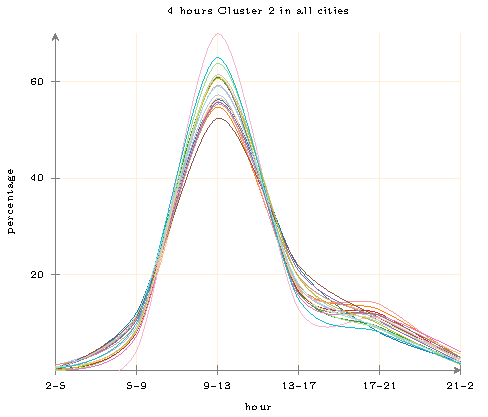
\includegraphics[height=0.18\textheight]{cluster_day_4h_cl2}}{\begin{tikzpicture}
	\begin{axis}[%
            title={ 4 hours Cluster 2 in all cities},
            xlabel={hour},
            ylabel={percentage},
            grid=major,
            xticklabels={,2--5,5--9,9--13,13--17,17--21,21--2}
		]
\addplot[ck1, thin, smooth] table[x index=0, y index=2] {amsterdam_cluster_day_4h.dat};
\addplot[ck2, thin, smooth,] table[x index=0, y index=2]{atlanta_cluster_day_4h.dat};
\addplot[ck3, thin, smooth,] table[x index=0, y index=2]{barcelona_cluster_day_4h.dat};
\addplot[ck4, thin, smooth,] table[x index=0, y index=2]{berlin_cluster_day_4h.dat};
\addplot[ck5, thin, smooth,] table[x index=0, y index=2]{chicago_cluster_day_4h.dat};
\addplot[ck6, thin, smooth,] table[x index=0, y index=2]{helsinki_cluster_day_4h.dat};
\addplot[ck7, thin, smooth,] table[x index=0, y index=2]{houston_cluster_day_4h.dat};
\addplot[ck8, thin, smooth,] table[x index=0, y index=2]{indianapolis_cluster_day_4h.dat};
\addplot[ck9, thin, smooth,] table[x index=0, y index=2]{london_cluster_day_4h.dat};
\addplot[ck10, thin, smooth,] table[x index=0, y index=2]{losangeles_cluster_day_4h.dat};
\addplot[ck11, thin, smooth,] table[x index=0, y index=2]{moscow_cluster_day_4h.dat};
\addplot[ck12, thin, smooth,] table[x index=0, y index=2]{newyork_cluster_day_4h.dat};
\addplot[ck13, thin, smooth,] table[x index=0, y index=2]{paris_cluster_day_4h.dat};
\addplot[ck14, thin, smooth,] table[x index=0, y index=2]{prague_cluster_day_4h.dat};
\addplot[ck15, thin, smooth,] table[x index=0, y index=2]{rome_cluster_day_4h.dat};
\addplot[ck16, thin, smooth,] table[x index=0, y index=2]{sanfrancisco_cluster_day_4h.dat};
\addplot[ck17, thin, smooth,] table[x index=0, y index=2]{seattle_cluster_day_4h.dat};
\addplot[ck18, thin, smooth,] table[x index=0, y index=2]{stlouis_cluster_day_4h.dat};
\addplot[ck19, thin, smooth,] table[x index=0, y index=2]{stockholm_cluster_day_4h.dat};
\addplot[ck20, thin, smooth,] table[x index=0, y index=2]{washington_cluster_day_4h.dat};
\end{axis}
\end{tikzpicture}
}
    \end{subfigure}

    \begin{subfigure}[b]{0.35\textwidth}
    \centering
    \iftoggle{EXTERNALPGF}{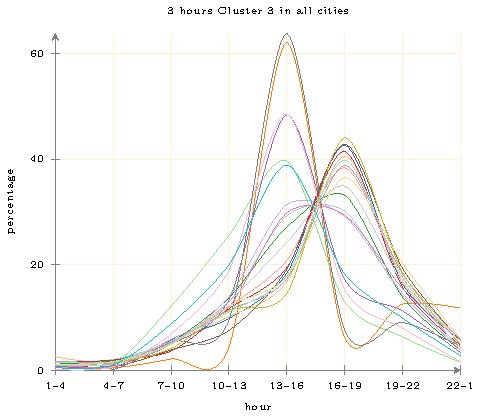
\includegraphics[height=0.18\textheight]{cluster_day_3h_cl3}}{\begin{tikzpicture}
	\begin{axis}[%
            title={3 hours Cluster 3 in all cities},
            xlabel={hour},
            ylabel={percentage},
            grid=major,
            xticklabels={,1--4, 4--7, 7--10, 10--13, 13--16, 16--19, 19--22, 22--1},
		]
\addplot[ck1, thin, smooth] table[x index=0, y index=3] {amsterdam_cluster_day_3h.dat};
\addplot[ck2, thin, smooth,] table[x index=0, y index=3]{atlanta_cluster_day_3h.dat};
\addplot[ck3, thin, smooth,] table[x index=0, y index=3]{barcelona_cluster_day_3h.dat};
\addplot[ck4, thin, smooth,] table[x index=0, y index=3]{berlin_cluster_day_3h.dat};
\addplot[ck5, thin, smooth,] table[x index=0, y index=3]{chicago_cluster_day_3h.dat};
\addplot[ck6, thin, smooth,] table[x index=0, y index=3]{helsinki_cluster_day_3h.dat};
\addplot[ck7, thin, smooth,] table[x index=0, y index=3]{houston_cluster_day_3h.dat};
\addplot[ck8, thin, smooth,] table[x index=0, y index=3]{indianapolis_cluster_day_3h.dat};
\addplot[ck9, thin, smooth,] table[x index=0, y index=3]{london_cluster_day_3h.dat};
\addplot[ck10, thin, smooth,] table[x index=0, y index=3]{losangeles_cluster_day_3h.dat};
\addplot[ck11, thin, smooth,] table[x index=0, y index=3]{moscow_cluster_day_3h.dat};
\addplot[ck12, thin, smooth,] table[x index=0, y index=3]{newyork_cluster_day_3h.dat};
\addplot[ck13, thin, smooth,] table[x index=0, y index=3]{paris_cluster_day_3h.dat};
\addplot[ck14, thin, smooth,] table[x index=0, y index=3]{prague_cluster_day_3h.dat};
\addplot[ck15, thin, smooth,] table[x index=0, y index=3]{rome_cluster_day_3h.dat};
\addplot[ck16, thin, smooth,] table[x index=0, y index=3]{sanfrancisco_cluster_day_3h.dat};
\addplot[ck17, thin, smooth,] table[x index=0, y index=3]{seattle_cluster_day_3h.dat};
\addplot[ck18, thin, smooth,] table[x index=0, y index=3]{stlouis_cluster_day_3h.dat};
\addplot[ck19, thin, smooth,] table[x index=0, y index=3]{stockholm_cluster_day_3h.dat};
\addplot[ck20, thin, smooth,] table[x index=0, y index=3]{washington_cluster_day_3h.dat};
\end{axis}
\end{tikzpicture}
}
    \end{subfigure}~
    \begin{subfigure}[b]{0.35\textwidth}
    \centering
    \iftoggle{EXTERNALPGF}{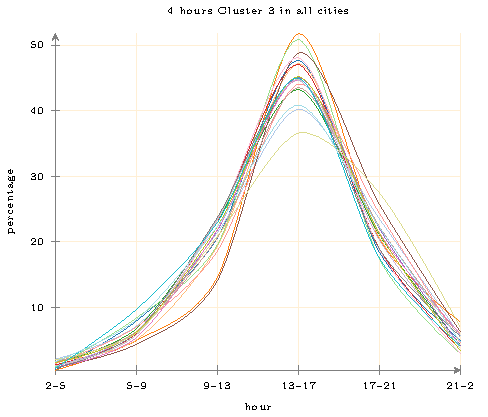
\includegraphics[height=0.18\textheight]{cluster_day_4h_cl3}}{\begin{tikzpicture}
	\begin{axis}[%
            title={ 4 hours Cluster 3 in all cities},
            xlabel={hour},
            ylabel={percentage},
            grid=major,
            xticklabels={,2--5,5--9,9--13,13--17,17--21,21--2}
		]
\addplot[ck1, thin, smooth] table[x index=0, y index=3] {amsterdam_cluster_day_4h.dat};
\addplot[ck2, thin, smooth,] table[x index=0, y index=3]{atlanta_cluster_day_4h.dat};
\addplot[ck3, thin, smooth,] table[x index=0, y index=3]{barcelona_cluster_day_4h.dat};
\addplot[ck4, thin, smooth,] table[x index=0, y index=3]{berlin_cluster_day_4h.dat};
\addplot[ck5, thin, smooth,] table[x index=0, y index=3]{chicago_cluster_day_4h.dat};
\addplot[ck6, thin, smooth,] table[x index=0, y index=3]{helsinki_cluster_day_4h.dat};
\addplot[ck7, thin, smooth,] table[x index=0, y index=3]{houston_cluster_day_4h.dat};
\addplot[ck8, thin, smooth,] table[x index=0, y index=3]{indianapolis_cluster_day_4h.dat};
\addplot[ck9, thin, smooth,] table[x index=0, y index=3]{london_cluster_day_4h.dat};
\addplot[ck10, thin, smooth,] table[x index=0, y index=3]{losangeles_cluster_day_4h.dat};
\addplot[ck11, thin, smooth,] table[x index=0, y index=3]{moscow_cluster_day_4h.dat};
\addplot[ck12, thin, smooth,] table[x index=0, y index=3]{newyork_cluster_day_4h.dat};
\addplot[ck13, thin, smooth,] table[x index=0, y index=3]{paris_cluster_day_4h.dat};
\addplot[ck14, thin, smooth,] table[x index=0, y index=3]{prague_cluster_day_4h.dat};
\addplot[ck15, thin, smooth,] table[x index=0, y index=3]{rome_cluster_day_4h.dat};
\addplot[ck16, thin, smooth,] table[x index=0, y index=3]{sanfrancisco_cluster_day_4h.dat};
\addplot[ck17, thin, smooth,] table[x index=0, y index=3]{seattle_cluster_day_4h.dat};
\addplot[ck18, thin, smooth,] table[x index=0, y index=3]{stlouis_cluster_day_4h.dat};
\addplot[ck19, thin, smooth,] table[x index=0, y index=3]{stockholm_cluster_day_4h.dat};
\addplot[ck20, thin, smooth,] table[x index=0, y index=3]{washington_cluster_day_4h.dat};
\end{axis}
\end{tikzpicture}
}
    \end{subfigure}

    \begin{subfigure}[b]{0.35\textwidth}
    \centering
    \iftoggle{EXTERNALPGF}{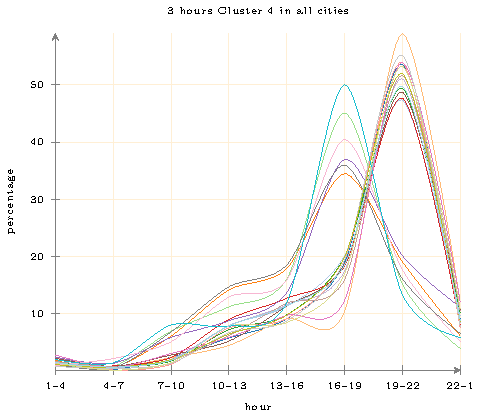
\includegraphics[height=0.18\textheight]{cluster_day_3h_cl4}}{\begin{tikzpicture}
	\begin{axis}[%
            title={3 hours Cluster 4 in all cities},
            xlabel={hour},
            ylabel={percentage},
            grid=major,
            xticklabels={,1--4, 4--7, 7--10, 10--13, 13--16, 16--19, 19--22, 22--1},
		]
\addplot[ck1, thin, smooth] table[x index=0, y index=4] {amsterdam_cluster_day_3h.dat};
\addplot[ck2, thin, smooth,] table[x index=0, y index=4]{atlanta_cluster_day_3h.dat};
\addplot[ck3, thin, smooth,] table[x index=0, y index=4]{barcelona_cluster_day_3h.dat};
\addplot[ck4, thin, smooth,] table[x index=0, y index=4]{berlin_cluster_day_3h.dat};
\addplot[ck5, thin, smooth,] table[x index=0, y index=4]{chicago_cluster_day_3h.dat};
\addplot[ck6, thin, smooth,] table[x index=0, y index=4]{helsinki_cluster_day_3h.dat};
\addplot[ck7, thin, smooth,] table[x index=0, y index=4]{houston_cluster_day_3h.dat};
\addplot[ck8, thin, smooth,] table[x index=0, y index=4]{indianapolis_cluster_day_3h.dat};
\addplot[ck9, thin, smooth,] table[x index=0, y index=4]{london_cluster_day_3h.dat};
\addplot[ck10, thin, smooth,] table[x index=0, y index=4]{losangeles_cluster_day_3h.dat};
\addplot[ck11, thin, smooth,] table[x index=0, y index=4]{moscow_cluster_day_3h.dat};
\addplot[ck12, thin, smooth,] table[x index=0, y index=4]{newyork_cluster_day_3h.dat};
\addplot[ck13, thin, smooth,] table[x index=0, y index=4]{paris_cluster_day_3h.dat};
\addplot[ck14, thin, smooth,] table[x index=0, y index=4]{prague_cluster_day_3h.dat};
\addplot[ck15, thin, smooth,] table[x index=0, y index=4]{rome_cluster_day_3h.dat};
\addplot[ck16, thin, smooth,] table[x index=0, y index=4]{sanfrancisco_cluster_day_3h.dat};
\addplot[ck17, thin, smooth,] table[x index=0, y index=4]{seattle_cluster_day_3h.dat};
\addplot[ck18, thin, smooth,] table[x index=0, y index=4]{stlouis_cluster_day_3h.dat};
\addplot[ck19, thin, smooth,] table[x index=0, y index=4]{stockholm_cluster_day_3h.dat};
\addplot[ck20, thin, smooth,] table[x index=0, y index=4]{washington_cluster_day_3h.dat};
\end{axis}
\end{tikzpicture}
}
    \end{subfigure}~
    \begin{subfigure}[b]{0.35\textwidth}
    \centering
    \iftoggle{EXTERNALPGF}{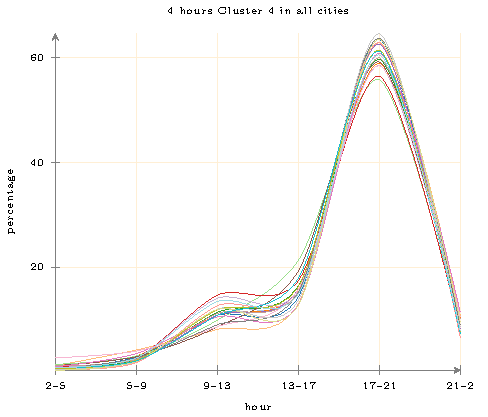
\includegraphics[height=0.18\textheight]{cluster_day_4h_cl4}}{\begin{tikzpicture}
	\begin{axis}[%
            title={ 4 hours Cluster 4 in all cities},
            xlabel={hour},
            ylabel={percentage},
            grid=major,
            xticklabels={,2--5,5--9,9--13,13--17,17--21,21--2}
		]
\addplot[ck1, thin, smooth] table[x index=0, y index=4] {amsterdam_cluster_day_4h.dat};
\addplot[ck2, thin, smooth,] table[x index=0, y index=4]{atlanta_cluster_day_4h.dat};
\addplot[ck3, thin, smooth,] table[x index=0, y index=4]{barcelona_cluster_day_4h.dat};
\addplot[ck4, thin, smooth,] table[x index=0, y index=4]{berlin_cluster_day_4h.dat};
\addplot[ck5, thin, smooth,] table[x index=0, y index=4]{chicago_cluster_day_4h.dat};
\addplot[ck6, thin, smooth,] table[x index=0, y index=4]{helsinki_cluster_day_4h.dat};
\addplot[ck7, thin, smooth,] table[x index=0, y index=4]{houston_cluster_day_4h.dat};
\addplot[ck8, thin, smooth,] table[x index=0, y index=4]{indianapolis_cluster_day_4h.dat};
\addplot[ck9, thin, smooth,] table[x index=0, y index=4]{london_cluster_day_4h.dat};
\addplot[ck10, thin, smooth,] table[x index=0, y index=4]{losangeles_cluster_day_4h.dat};
\addplot[ck11, thin, smooth,] table[x index=0, y index=4]{moscow_cluster_day_4h.dat};
\addplot[ck12, thin, smooth,] table[x index=0, y index=4]{newyork_cluster_day_4h.dat};
\addplot[ck13, thin, smooth,] table[x index=0, y index=4]{paris_cluster_day_4h.dat};
\addplot[ck14, thin, smooth,] table[x index=0, y index=4]{prague_cluster_day_4h.dat};
\addplot[ck15, thin, smooth,] table[x index=0, y index=4]{rome_cluster_day_4h.dat};
\addplot[ck16, thin, smooth,] table[x index=0, y index=4]{sanfrancisco_cluster_day_4h.dat};
\addplot[ck17, thin, smooth,] table[x index=0, y index=4]{seattle_cluster_day_4h.dat};
\addplot[ck18, thin, smooth,] table[x index=0, y index=4]{stlouis_cluster_day_4h.dat};
\addplot[ck19, thin, smooth,] table[x index=0, y index=4]{stockholm_cluster_day_4h.dat};
\addplot[ck20, thin, smooth,] table[x index=0, y index=4]{washington_cluster_day_4h.dat};
\end{axis}
\end{tikzpicture}
}
    \end{subfigure}

    \begin{subfigure}[b]{0.35\textwidth}
    \centering
    \iftoggle{EXTERNALPGF}{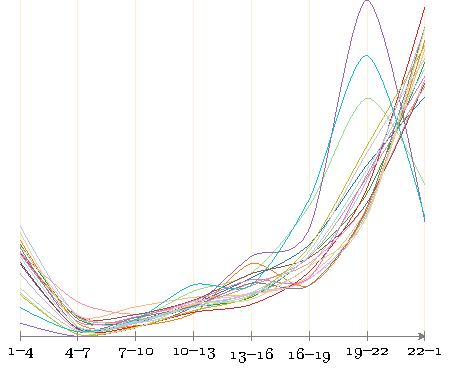
\includegraphics[height=0.18\textheight]{cluster_day_3h_cl5}}{\begin{tikzpicture}
	\begin{axis}[%
			axis y line=none,
            % title={3 hours Cluster 5 in all cities},
            % xlabel={hour},
            % ylabel={percentage},
            grid=major,
            xticklabels={,1--4, 4--7, 7--10, 10--13, 13--16, 16--19, 19--22, 22--1},
		]
\addplot[ck1, thin, smooth] table[x index=0, y index=5] {amsterdam_cluster_day_3h.dat};
\addplot[ck2, thin, smooth,] table[x index=0, y index=5]{atlanta_cluster_day_3h.dat};
\addplot[ck3, thin, smooth,] table[x index=0, y index=5]{barcelona_cluster_day_3h.dat};
\addplot[ck4, thin, smooth,] table[x index=0, y index=5]{berlin_cluster_day_3h.dat};
\addplot[ck5, thin, smooth,] table[x index=0, y index=5]{chicago_cluster_day_3h.dat};
\addplot[ck6, thin, smooth,] table[x index=0, y index=5]{helsinki_cluster_day_3h.dat};
\addplot[ck7, thin, smooth,] table[x index=0, y index=5]{houston_cluster_day_3h.dat};
\addplot[ck8, thin, smooth,] table[x index=0, y index=5]{indianapolis_cluster_day_3h.dat};
\addplot[ck9, thin, smooth,] table[x index=0, y index=5]{london_cluster_day_3h.dat};
\addplot[ck10, thin, smooth,] table[x index=0, y index=5]{losangeles_cluster_day_3h.dat};
\addplot[ck11, thin, smooth,] table[x index=0, y index=5]{moscow_cluster_day_3h.dat};
\addplot[ck12, thin, smooth,] table[x index=0, y index=5]{newyork_cluster_day_3h.dat};
\addplot[ck13, thin, smooth,] table[x index=0, y index=5]{paris_cluster_day_3h.dat};
\addplot[ck14, thin, smooth,] table[x index=0, y index=5]{prague_cluster_day_3h.dat};
\addplot[ck15, thin, smooth,] table[x index=0, y index=5]{rome_cluster_day_3h.dat};
\addplot[ck16, thin, smooth,] table[x index=0, y index=5]{sanfrancisco_cluster_day_3h.dat};
\addplot[ck17, thin, smooth,] table[x index=0, y index=5]{seattle_cluster_day_3h.dat};
\addplot[ck18, thin, smooth,] table[x index=0, y index=5]{stlouis_cluster_day_3h.dat};
\addplot[ck19, thin, smooth,] table[x index=0, y index=5]{stockholm_cluster_day_3h.dat};
\addplot[ck20, thin, smooth,] table[x index=0, y index=5]{washington_cluster_day_3h.dat};
\end{axis}
\end{tikzpicture}
}
    \end{subfigure}~
    \begin{subfigure}[b]{0.35\textwidth}
    \centering
    \iftoggle{EXTERNALPGF}{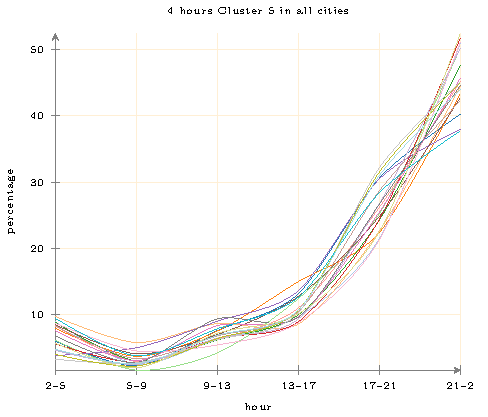
\includegraphics[height=0.18\textheight]{cluster_day_4h_cl5}}{\begin{tikzpicture}
	\begin{axis}[%
			axis y line=none,
            grid=major,
            xticklabels={,2--5,5--9,9--13,13--17,17--21,21--2}
		]
\addplot[ck1, thin, smooth] table[x index=0, y index=5] {amsterdam_cluster_day_4h.dat};
\addplot[ck2, thin, smooth,] table[x index=0, y index=5]{atlanta_cluster_day_4h.dat};
\addplot[ck3, thin, smooth,] table[x index=0, y index=5]{barcelona_cluster_day_4h.dat};
\addplot[ck4, thin, smooth,] table[x index=0, y index=5]{berlin_cluster_day_4h.dat};
\addplot[ck5, thin, smooth,] table[x index=0, y index=5]{chicago_cluster_day_4h.dat};
\addplot[ck6, thin, smooth,] table[x index=0, y index=5]{helsinki_cluster_day_4h.dat};
\addplot[ck7, thin, smooth,] table[x index=0, y index=5]{houston_cluster_day_4h.dat};
\addplot[ck8, thin, smooth,] table[x index=0, y index=5]{indianapolis_cluster_day_4h.dat};
\addplot[ck9, thin, smooth,] table[x index=0, y index=5]{london_cluster_day_4h.dat};
\addplot[ck10, thin, smooth,] table[x index=0, y index=5]{losangeles_cluster_day_4h.dat};
\addplot[ck11, thin, smooth,] table[x index=0, y index=5]{moscow_cluster_day_4h.dat};
\addplot[ck12, thin, smooth,] table[x index=0, y index=5]{newyork_cluster_day_4h.dat};
\addplot[ck13, thin, smooth,] table[x index=0, y index=5]{paris_cluster_day_4h.dat};
\addplot[ck14, thin, smooth,] table[x index=0, y index=5]{prague_cluster_day_4h.dat};
\addplot[ck15, thin, smooth,] table[x index=0, y index=5]{rome_cluster_day_4h.dat};
\addplot[ck16, thin, smooth,] table[x index=0, y index=5]{sanfrancisco_cluster_day_4h.dat};
\addplot[ck17, thin, smooth,] table[x index=0, y index=5]{seattle_cluster_day_4h.dat};
\addplot[ck18, thin, smooth,] table[x index=0, y index=5]{stlouis_cluster_day_4h.dat};
\addplot[ck19, thin, smooth,] table[x index=0, y index=5]{stockholm_cluster_day_4h.dat};
\addplot[ck20, thin, smooth,] table[x index=0, y index=5]{washington_cluster_day_4h.dat};
\end{axis}
\end{tikzpicture}
}
    \end{subfigure}
    \caption[Venues cluster by time among all the cities]{
		Results of $k$-means with $k=5$ on the 3-hours window (left column) and 4-hours window (right column) check-in distribution of venues. 
Each line in each figure is the centroid of a cluster in a city.\label{fig:time_cluster_size}}
\end{figure}
\clearpage
\restoregeometry

\subsection{Space}

The other main characteristic of every check-in is where it takes place. We
focus on two spatial feature of venues. First, was does the surrounding looks
like in terms of categories. For instance, if a restaurant is mainly
surrounded by night life places and another by education buildings, they
probably have different customers. Second, venues are not uniformly
distributed within the city and the density of nearby locations is a
discriminative feature as well. For instance in \autoref{fig:density_paris},
we can clearly distinguish venues belonging to the city center from the
others.

\begin{figure}[h]
        \centering
    \begin{subfigure}[b]{0.32\textheight}
        \centering
        \includegraphics[width=\textwidth]{paris_new_density_50.pdf}
    \end{subfigure}
    \begin{subfigure}[b]{0.32\textheight}
	\includegraphics[width=\textwidth]{paris_new_density_160.pdf}
    \end{subfigure}
    \begin{subfigure}[b]{0.32\textheight}
        \centering
	\includegraphics[width=\textwidth]{paris_new_density_350.pdf}
    \end{subfigure}
\caption[Venue density in Paris]{Estimated density of 3192 venues in Paris by a
Gaussian kernel. On the top, the bandwidth is 50 meters and it looks too small:
venues are isolated. In the middle, $h=160$ because this value maximize the
probability of existing venues.  On the bottom, $h=350$ corresponds to human
definition of neighborhood size.\label{fig:density_paris}}
\end{figure}

\subsection{Location entropy}

\Textcite{Entropy10} showed that \enquote{location entropy, which measures the
diversity of unique visitors of a location} gives good indication of the
sociability level of venues and therefore help predicting friendship ties within
\gls{lbsn}.

Let $\mathcal{U}$ be the set of users and $\mathcal{V}$ the one of venues. For
each venue $v \in \mathcal{V}$, we can gather the set of check-ins $c_v$ that
occurred there as well as the corresponding users $[u_1, u_2, u_2, \ldots,
u_n]$ (note that the same users can check-in multiple times). Then we
transform this list to a frequency distribution $f_v$ over $\mathcal{U}$ and
compute the normalized entropy: \[
    H(v) = -\frac{1}{\log\left(\left| \mathcal{U}\right|\right)}
\sum_{u\in \mathcal{U}} f_v(u) \log(f_v(u)) \]

Computing this value for all venues in Paris and Barcelona shows that it is a
good descriptor of the \enquote{publicness} of a place. As showed in
\autoref{tab:entropy}, touristic attractions like the Sagrada Família or the
Eiffel Tower exhibit high entropy because they are visited by a large and
diverse set of people. On the other hand, work offices and private houses have
low entropy, as they attract a much more restricted crowd.

\begin{table}[ht]
	\centering
\begin{tabular}{lllr}
	\toprule
	City                       & Name                           & Category                 & Entropy \\
	\midrule
	\multirow{3}{*}{Barcelona} & Castellers de Barcelona        & Non-Profit               & $0.0139$ \\
	                           & Café de la Pompeu              & Café                     & $0.0172$ \\
	                           & Ràdio 4                        & Radio Station            & $0.0176$ \\
	%                          & La Comarca                     & Home (private)           & $0.0180$ \\
	%                          & House castellar                & Home (private)           & $0.0181$ \\
	%                          & Av Tomas Gimenez               & Bar                      & $0.0186$ \\
	%                          & Torre De Barad-Dur             & Building                 & $0.0192$ \\
	\midrule
	\multirow{3}{*}{Paris}     & Blue Acacia                    & Office                   & $0.0119$ \\
	                           & Boutique Orange                & Electronics Store        & $0.0141$ \\
	                           & Regus                          & Office                   & $0.0163$ \\
	%                          & Café Pierre                    & French Restaurant        & $0.0181$ \\
	%                          & my home 2                      & Home (private)           & $0.0193$ \\
	%                          & 10e arrondissement – Entrepôt  & States \& Municipalities & $0.0213$ \\
	%                          & Scanblog                       & Office                   & $0.0221$ \\
	\midrule
	%                          & Parc de la Ciutadella          & Park                     & $0.5188$ \\
	%                          & Apple Store                    & Electronics Store        & $0.5358$ \\
	%                          & Parc Güell                     & Park                     & $0.5666$ \\
	\multirow{4}{*}{Barcelona} & Plaça de Catalunya             & Plaza                    & $0.5835$ \\
	                           & Sants Estació                  & Train Station            & $0.6298$ \\
	                           & Sagrada Família                & Government Building      & $0.6309$ \\
	                           & Camp Nou                       & Stadium                  & $0.6852$ \\
	\midrule
	%                          & Arc de Triomphe                & Government Building      & $0.5831$ \\
	%                          & Cathédrale Notre-Dame de Paris & Spiritual Center         & $0.5874$ \\
	%                          & Gare SNCF Paris Montparnasse   & Train Station            & $0.6141$ \\
	\multirow{4}{*}{Paris}     & Musée du Louvre                & Museum                   & $0.6444$ \\
	                           & Gare SNCF Gare de Lyon         & Train Station            & $0.6460$ \\
	                           & Tour Eiffel                    & Government Building      & $0.6618$ \\
	                           & Gare SNCF Paris Nord           & Train Station            & $0.6707$ \\
	\bottomrule
\end{tabular}
\caption{Venues in Paris and Barcelona with lowest and highest user
entropy.\label{tab:entropy}}
\end{table}

Following the same idea, we also computed the entropy of locations with respect
to time of check-ins. Indeed, it distinguishes between a railway station active
all day long and a restaurant open only during lunch hours.  We also expect a
link between the two entropies, as places that stay open longer have more
chance to be visited by a various set of users. But this relation, shown on
\autoref{fig:two_entropies}[REDRAW IT] is weak, as some places are visited all the time by
a small group of dedicated people.

\begin{figure}[hbtp]
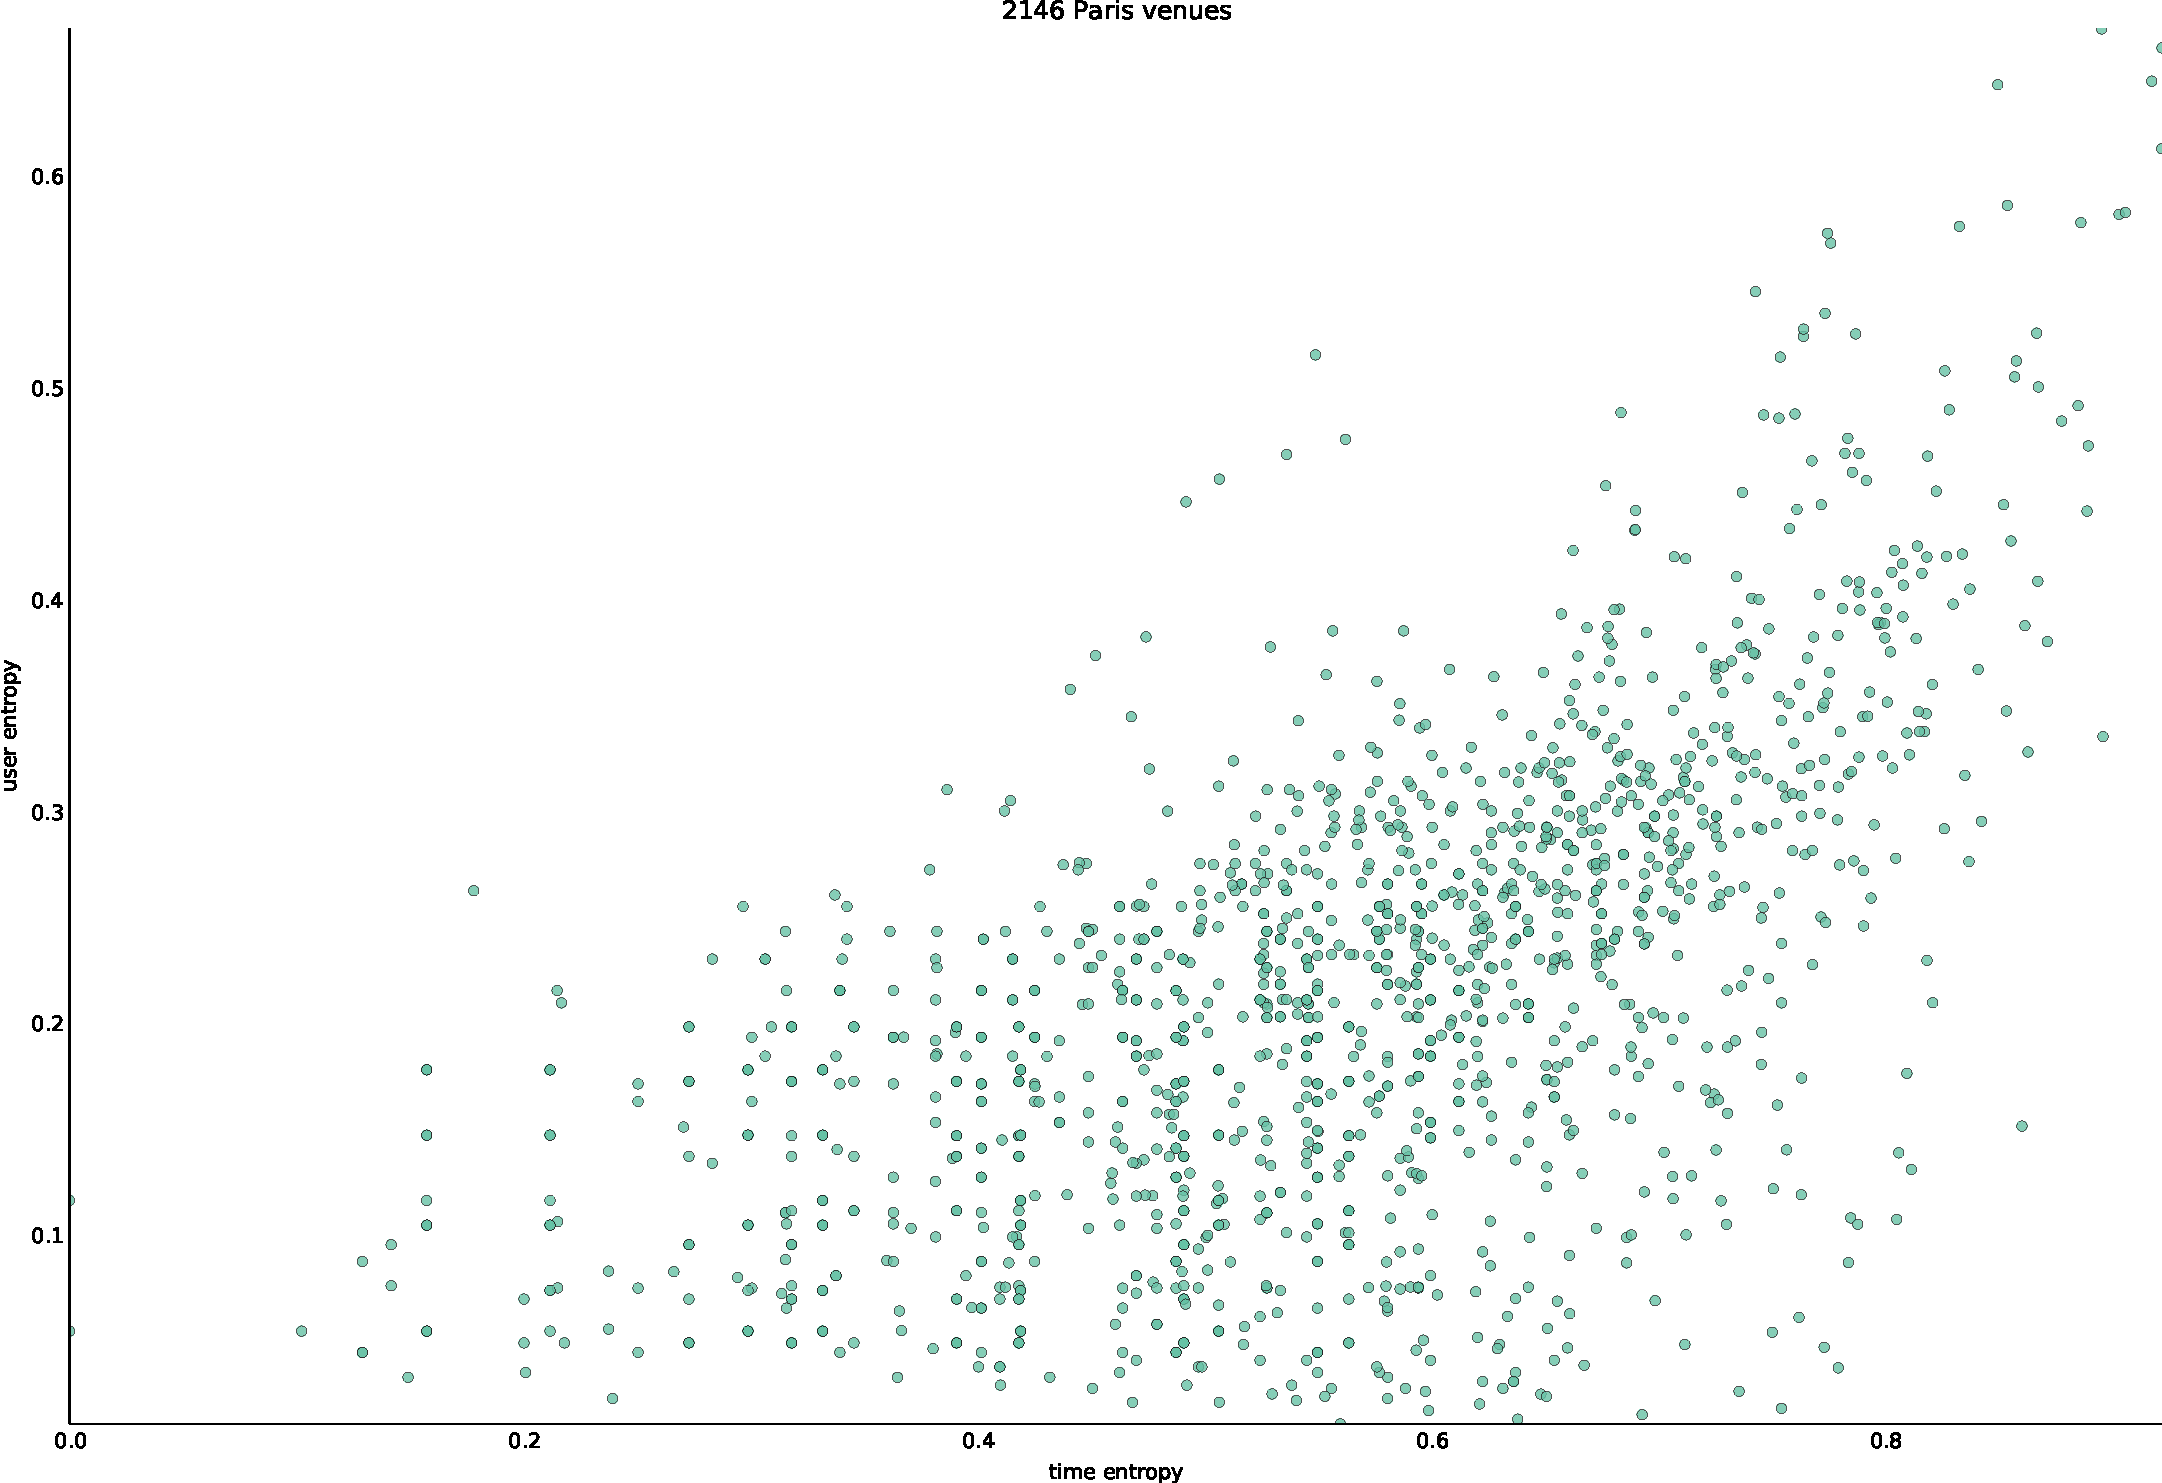
\includegraphics[width=\textwidth]{two_entropies}
\caption{Venues entropy with respect to user population and time of check-in
during the day. \label{fig:two_entropies}}
\end{figure}


\subsection{Photos}

Finally, one interesting aspect of this dataset is the interaction between
check-ins and photos.  The spatial repartition of both objects can be seen as
an indirect signal of interest within the city. Thus we were curious to see in
which place they disagree, that is location where there is significantly more
photos taken that what we would expect by looking at the tweet concentration
(and conversely). To answer this question, we compute the discrepancy between
this two measure of activity \autocite{Agarwal2006spatial}. It turns out that
some places are mostly checked-in because events take place there (such as when
people arrive in a new city via a railway station or an airport, or when a
sport team plays a match in a stadium) whereas other are more photographed,
like museum or touristic sights.

% Look at high and low focus places: not so interesting either. High value are
% for popular places like park or monument whereas low (but not zero) are for
% mundane place (like pizzeria) close to famous locations.
